\documentclass{article}
\usepackage[utf8]{inputenc}

\title{My first open source contribution.}
\author{Marietta Lazana - t8160057@aueb.gr}
\date{May 2019}

\begin{document}

\maketitle

% Here is the abstract.
\begin{abstract}
The attempt to contribute to an open source project has proven to be extremely beneficial. It, greatly, reduced inhibitory factors by demystifying the contributory process. Personally, it was a challenge, to examine my abilities and strengths in a quite big and very fast moving project. Facing the real world of Software Engineering was surely a great experience!
  
\end{abstract}
%---

\section*{Introduction}
The "Software Engineering in Practise" course is one of the most important in my undergraduate degree, since it has prompted me to gain my first serious experience in this field. Under the supervision of the professor Diomidis Spinellis and the help of PhD candidate Antonis Gkortzis I gained useful knowledge in software engineering that helped me produce as much professional code as I could at this time. I learned about software design, construction, testing, maintenance, management and more, following the book of IEEE "SWEBOK, Software Engineering  Body of Knowledge". Last but not least, I gained a better understanding of git that helped me work on the open source project I chose.

\section{Project Understanding}


\includegraphics[width = 40mm]{logo}

I had two criteria while searching for a project. The first was high difficulty and the second was to be something that will enthusiasm me. So when I found ArchiveBox I thought that it was a great idea and also when I start reading the code I didn't understand anything. So I was sure that this was going to be a project that will definately help me improve.

ArchiveBox[1] is a very promising and upcoming project created by Nick Sweeting (GitHub: pirate) and has a vision of archiving everything from the internet. It is motivated by the fact that many people find interesting information on the internet that want to store locally, and most importantly, in multiple redundant common formats(HTML, PDF, PNG, WARC etc.). So, the user gives specific terminal commands including the URL that wants to archive, and then all the formats of the archived website are stored and organized in an HTML page.

While trying to build the project I faced a very basic problem. My operating system (Windows) couldn't support the project. So I came up with the solution of working from a virtual machine that runs on Linux, more precisely I worked with Oracle's VM, virtualbox. 

Finally, in order to understand deeper the project I started reading the code of every file and categorize it depending on its role. Of course, the documentation helped me a lot in this process.


\section{My contribution}

At first, I was trying to find something that I could contribute. Luckily, the person who ones repository, Nick, mentioned me in a issue with medium difficulty.
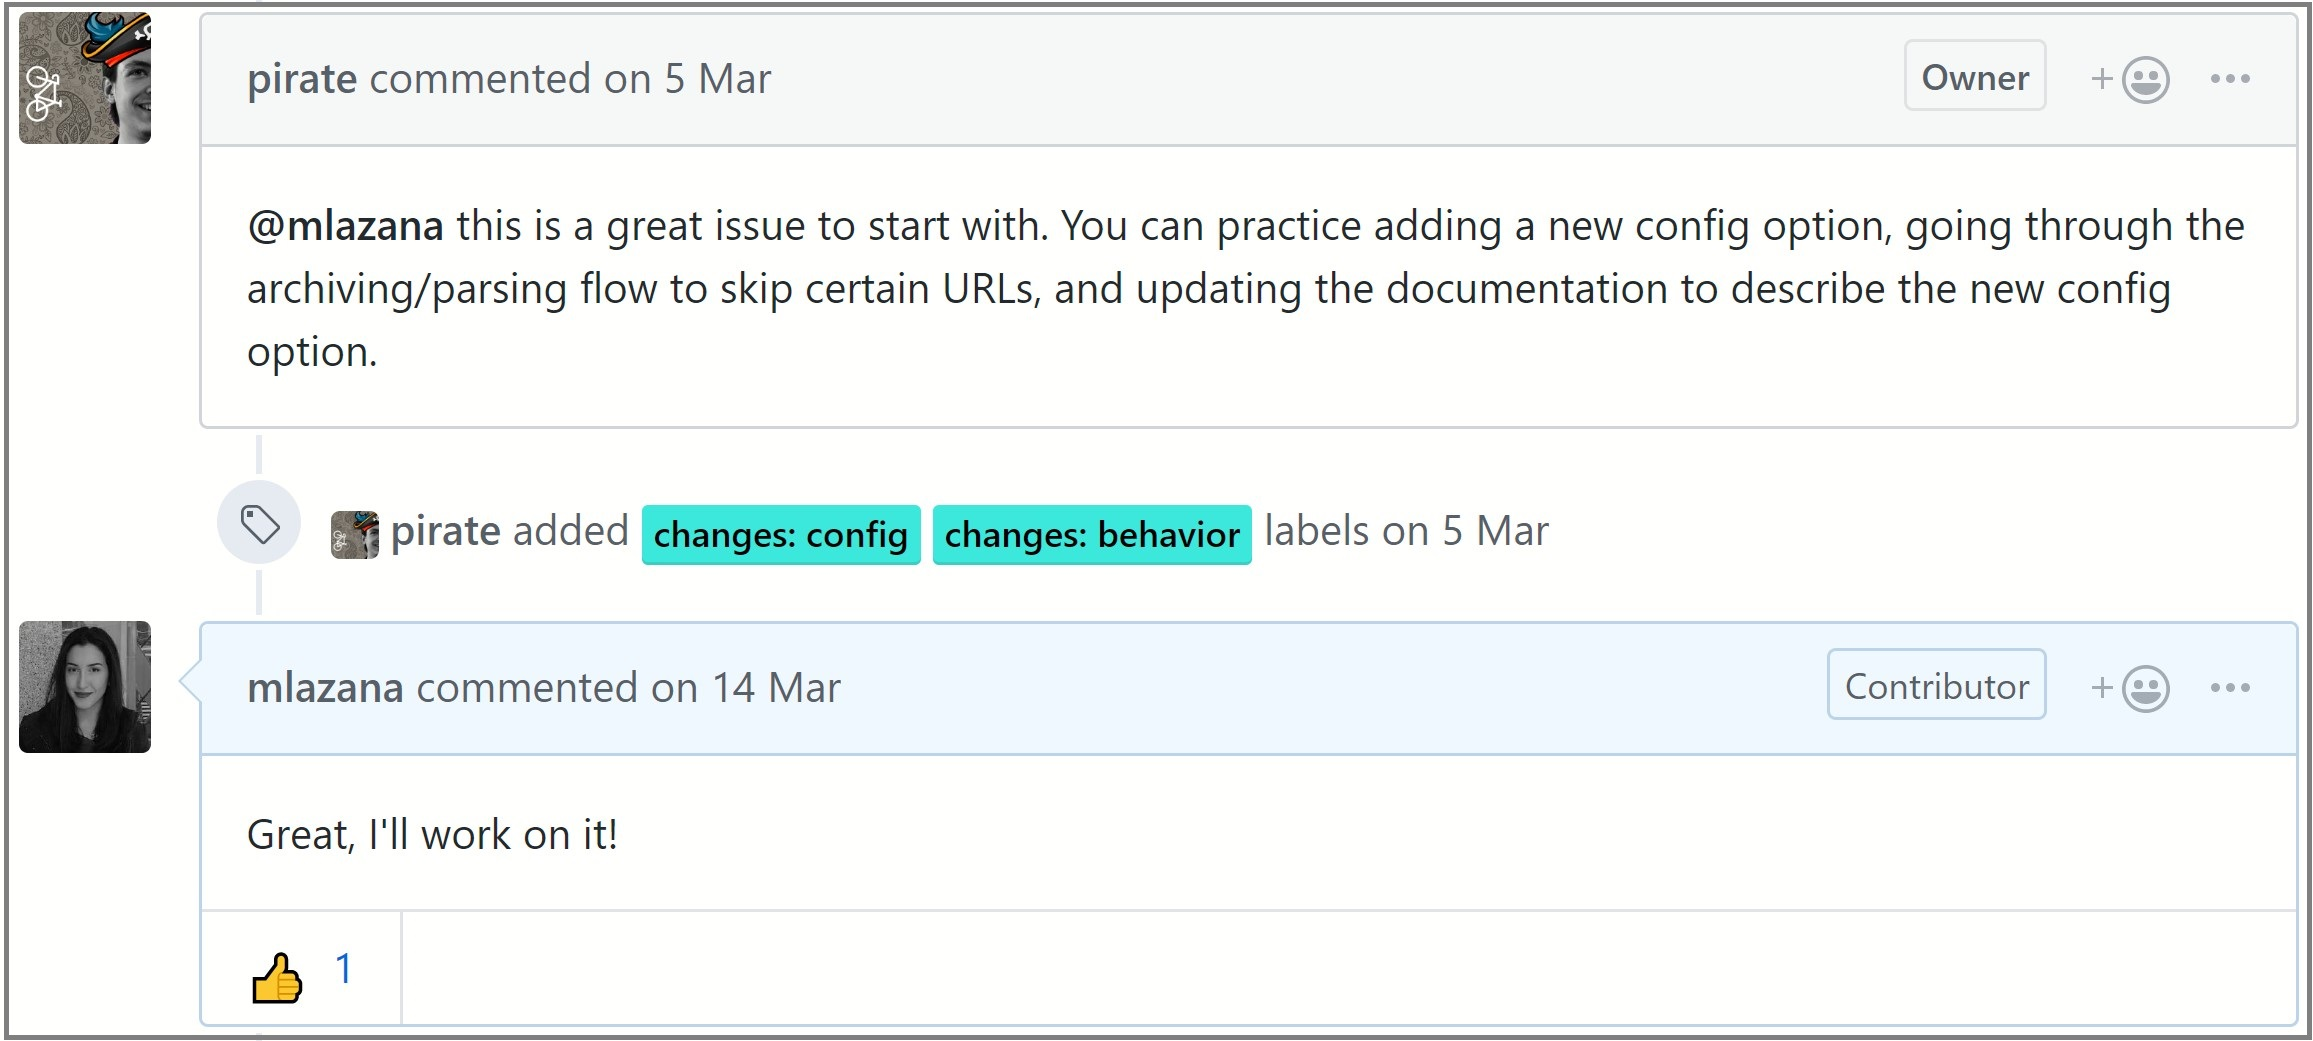
\includegraphics[width = 40mm]{mention}
That was very good for me because I needed to break out of my comfort zone and deal with a problem I didn't choose.

The issue was that needed to be closed was about creating a blacklist of URLs that shouldn't be archived. For example, in many cases bookmarks included websites that were useless in terms of archiving. So when someone wanted to archive his bookmarks he would have also unimportant information, using disk space.

My first step while dealing with this issue was to understand which parts of the code were producing the archiving/parsing flow. So, I found the specific files that are involved with this process and start experimenting by changing part of its so that I could understand what I needed to do. My thought was to create a method as a filter in order to check which URLs are the proper ones. 
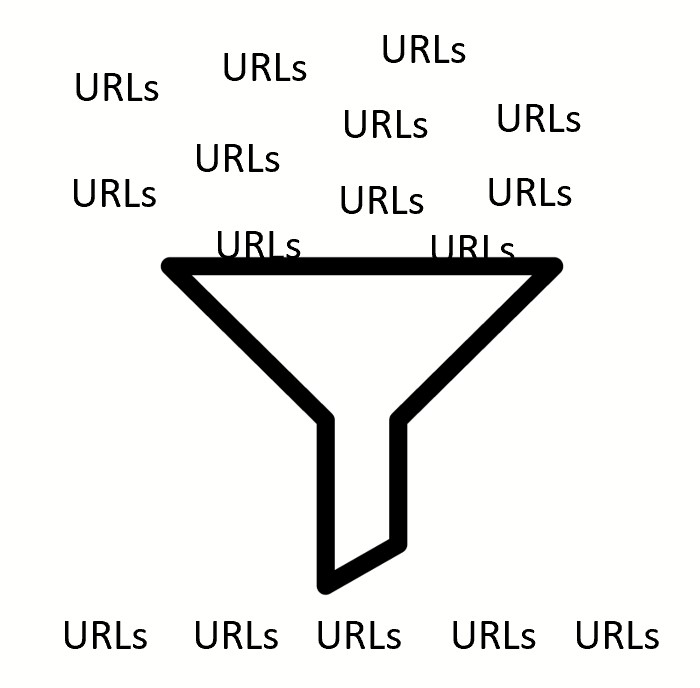
\includegraphics[width = 40mm]{filter}

Before that I loaded an environment variable and used the method re.compile() to compile the regex.
\begin{center}
\begin{verbatim}

URL_BLACKLIST = re.compile(
    r'(.*\.youtube\.com)|'
    r'(.*\.amazon\.com)|'
    r'(.*\.reddit\.com)',
    re.IGNORECASE,
    ) 
\end{verbatim}
\end{center}

After that I created a method to exclude any URL that was in blacklist using generator comprehensions. 
\begin{verbatim}
def exclude_blacklisted(links):
    """exclude URLs that match the blacklisted url pattern regex"""
    return (link for link in links if not URL_BLACKLIST.match(link['url']))
\end{verbatim}

Finally, I had one more challenge. I needed to find the perfect place to call this method, as links can only get loaded in a couple of places. Adding links from a new import source, parsing an existing output/links.json index file, or reading an individual output/archive/<ts>/index.json file.
So, I found a method which is executed before these three methods are called. 

\subsection{Code quality}

First of all, in the begging of my contribution process I tried to read as much code as I could in order to understand the best practises. I detected what kind of names they give to their methods and variables, spaces and number of empty lines they use between their methods etc. I did that, as I wanted to contribute code that suits the project.

Further more, I wrote descriptive comments to my methods and variables. 
\begin{verbatim}
links = list(exclude_blacklisted(links))  # exclude URLs that match
the blacklisted url pattern regex
\end{verbatim}

I wrote in every method or variable I created, except in the ones that was very obvious what they were doing.

\subsection{Continuous Integration}
The project has only Docker Cloud (ci/dockercloud), which allows me to manage the project in a container without exposing it to the rest of my system. Eventually all my commits passed this check.

\includegraphics[]{}



\end{document}
